\documentclass[polish,polish,a4paper]{article}
\usepackage[T1]{fontenc}
\usepackage[utf8]{inputenc}
\usepackage{babel}
\usepackage{pslatex}
\usepackage{graphicx}
\usepackage{tikz}
\usepackage{pgfplots}
\usepackage{anysize}
\usepackage{pgfgantt}
\usepackage{latexsym,amsmath}
\marginsize{2.5cm}{2.5cm}{3cm}{3cm}


\newcommand{\name}[1]{\sffamily\bfseries\scriptsize #1}

\newcommand{\frontpage}[8]{
%% #1 - nazwa kursu
%% #2 - kierunek 
%% #3 - termin 
%% #4 - temat 
%% #5 - problem
%% #6 - skład grupy
%% #7 - nr grupy
%% #8 - data

\hfill
\includegraphics[width=4cm]{PWr.png}
\vspace{2cm}

\begin{tabular}{|p{0.72\textwidth}|p{0.28\textwidth}|}
\hline
\multicolumn{2}{|c|}{}\\
\multicolumn{2}{|c|}{{\LARGE #1}}\\
\multicolumn{2}{|c|}{}\\
\hline
\name{Kierunek} & \name{Termin}\\
\multicolumn{1}{|c|}{\textit{#2}} & \multicolumn{1}{|c|}{\textit{#3}} \\
\hline
\name{Temat} & \name{Problem}\\
\multicolumn{1}{|c|}{\textit{#4}} & \multicolumn{1}{|c|}{\textit{#5}} \\
\hline
\name{Skład grupy} & \name{Nr grupy}\\
\multicolumn{1}{|c|}{\textit{#6}} & \multicolumn{1}{|c|}{\textit{#7}} \\
\hline
\name{Prowadzący} & \name{data}\\
\multicolumn{1}{|c|}{\textit{Mgr inż. Radosław Idzikowski}} & \multicolumn{1}{|c|}{\textit{#8}} \\
\hline
\end{tabular}

}

\usepackage{listings}
\usepackage{xcolor} % for setting colors



% set the default code style
\lstset{
    frame=tb, % draw a frame at the top and bottom of the code block
    tabsize=4, % tab space width
    showstringspaces=false, % don't mark spaces in strings
    numbers=left, % display line numbers on the left
    commentstyle=\color{green}, % comment color
    keywordstyle=\color{blue}, % keyword color
    stringstyle=\color{red} % string color
}




\title{Sprawozdanie SPD}
\begin{document}
% #1 - nazwa kursu #2 - kierunek  #3 - termin #4 - temat #5 - problem #6 - skład grupy #7 - nr grupy #8 - data
\frontpage{Projektowanie Efektywnych Algorytmów}{Informatyka}{Piątek 13:15}{Metoda podzialu i ograniczen i/lub programowanie dynamiczne.}{WST}{200000 Adam Abacki,  20000 Bartosz Babacki}{1}{\today}
\pagestyle{empty}
\newpage
\section{Opis problemu}
Lorem ipsum dolor sit amet, consectetur adipiscing elit. Integer maximus sollicitudin neque ac ultricies. Duis convallis dui ac porta sollicitudin. Aliquam sagittis imperdiet neque, vitae congue sapien laoreet a\cite{Smut2012}. Morbi in augue at nisi pulvinar convallis. Donec rhoncus arcu at tortor venenatis aliquet. Proin sed sem a diam imperdiet sodales. Mauris semper velit volutpat orci placerat convallis id eget justo.

Sed quis orci nunc. Phasellus at viverra magna, sed ultricies dolor. Maecenas a turpis velit. Duis ligula nunc, consectetur nec ante vitae, maximus ullamcorper erat. Aliquam varius mollis dolor, eu porttitor mauris volutpat sed. Vestibulum eu mattis augue. Praesent quis nisi urna. Pellentesque habitant morbi tristique senectus et netus et malesuada fames ac turpis egestas. Nunc commodo vel sapien id semper. Mauris at mattis est. In vitae arcu vitae neque consectetur tempor. Mauris malesuada pellentesque congue.
\section{Metoda rozwiązania}
\subsection{Algorytm 1}
Aliquam porta scelerisque molestie. Nam hendrerit, purus quis consectetur consequat, sem ante molestie nulla, eu egestas nisi augue eget lacus. Duis pellentesque mattis risus ut feugiat. Praesent ut nunc nec nulla semper tempus. Sed id eleifend nulla, vestibulum accumsan nunc. Suspendisse malesuada nisi non risus fringilla, at tincidunt diam cursus. Vestibulum vel nisi at ligula scelerisque imperdiet a vitae turpis. Fusce consectetur gravida nisi, a vestibulum libero dictum nec . Fusce suscipit blandit magna eu sodales. Curabitur pharetra vel mauris et vulputate. Sed dolor leo, condimentum in rutrum vel, luctus a urna. Nulla facilisi. Mauris pulvinar erat volutpat mi laoreet posuere. Integer euismod eu neque quis iaculis. Maecenas et porttitor turpis.
\lstinputlisting[firstline = 3,caption=Algorytm Sortowania Bąbelkowego,language=C++]
{bubblesort.cpp}
\subsection{Algorytm 2}
Vestibulum nisl mauris, dignissim non ultrices eget, dignissim eu nunc. Nunc a lorem elit. Donec molestie, lorem at volutpat luctus, est ligula fringilla arcu, in ullamcorper justo diam et magna. Quisque commodo sem urna, in bibendum sem pretium quis. Proin pulvinar elementum ante, molestie aliquam eros laoreet quis. Donec faucibus ornare posuere. Nullam risus tortor, sollicitudin quis bibendum quis, dignissim et justo. Schemat widzimy na obrazku nr \ref{fig::sa}.
\begin{figure}
\centering
\input{sa}
\label{fig::sa}
\caption{Schemat algorytmu}
\end{figure}
\section{Eksperymenty obliczeniowe}
Obliczenia zastały wykonane na komputerze klasy PC z procesorem i7-6700K, kartą graficzną NVIDIA GeForce GTX 1080 SeaHawk, 16GB RAM i DYSK SSD. Jako miarę jakości algorytmu przyjęto średnie procentowe odchylenie (Percentage Relative Deviation, PRD) najlepszego otrzymanego rozwiązania $\pi$ względem rozwiązania referencyjnego $\pi^{ref}$:
\begin{equation}
PRD(\pi)=100\%(C_{max}(\pi)-C_{max}(\pi^{ref}))/C_{max}(\pi^{ref})
\end{equation}
Wszystkie wyniki zebrano i przedstawiono w tabeli nr \ref{tab:result} gdzie:
\begin{itemize}
\item $n$ - liczba zadań,
\item $PRD_{sortR}(\%)$ - średnie procentowe odchylenie dla algorytmu sortR,
\item $t_{sortR}(s)$ - czas dla algorytmu sortR,
\item itp.
\end{itemize}
\begin{table}[h!]
\centering
	\caption{Czas obliczeń oraz PRD dla ustalonej liczby iteracji.}
	\label{tab:result}
	{\begin{tabular}{cccccc}
		\hline
		$n$ &$optimum$&$PRD_{sortR}(\%)$ & $PRD_{2opt}(\%)$& $t_{sortR}(s)$& $t_{2opt}(s)$ \\
		\hline
        6   & & 4.9 & 4.9& 0.0049 & 0.0049 \\
		10  & & 6.5 & 6.7& 0.0105 & 0.0105 \\
		20  & & 6.1 & 6.4& 0.0207 & 0.0207 \\
		50  & & 4.8 & 4.4& 0.0750 & 0.0750 \\
		100 & & 6.9 & 6.4& 0.1543 & 0.1543 \\
		200 & & 7.6 & 7.1& 0.3136 & 0.3136 \\
		500 & & 2.5 & 1.7& 0.5902 & 0.5902 \\
		\hline
		\bf{Średnio}& & \bf{0.2225}& \bf{0.2225}& \bf{-5.54}& \bf{-4.34} \\
		\hline
	\end{tabular}}
	\end{table}
    \begin{figure}[h]
\centering
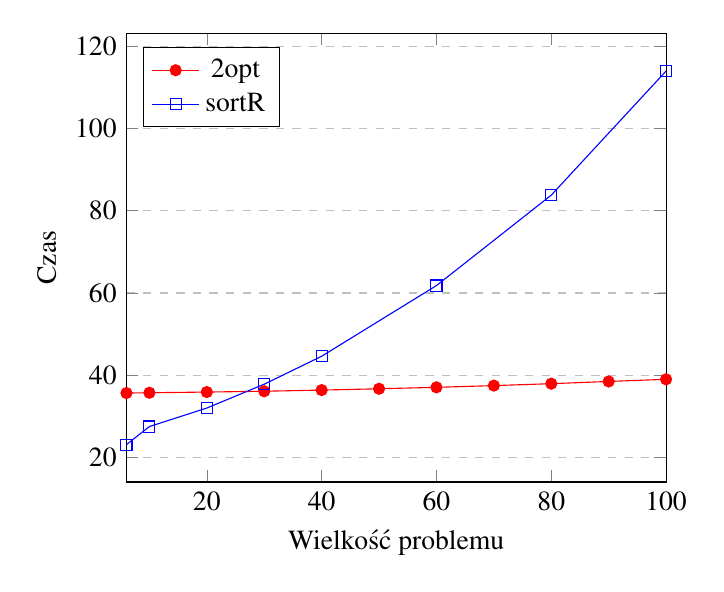
\begin{tikzpicture}
	\begin{axis}[
		xlabel=Wielkość problemu,
		ylabel=Czas,
        ymajorgrids=true,grid style=dashed,
        legend pos=north west,
        xmin=6,
        xmax=100
        ]
        \addplot[color=red,mark=*]
coordinates {
(6,35.65)
(10,35.72)
(20,35.89)
(30,36.09)
(40,36.37)
(50,36.69)
(60,37.04)
(70,37.46)
(80,37.93)
(90,38.47)
(100,38.99)
};

\addplot[color=blue,mark=square]
coordinates {
(6,23.1)
(10,27.5)
(20,32)
(30,37.8)
(40,44.6)
(60,61.8)
(80,83.8)
(100,114)
};
\legend{2opt,sortR}
	\end{axis}    
\end{tikzpicture}
\caption{Czas wykonywania się algorytmów w zależności od wielkości problemu}
\end{figure}
\section{Wnioski}
Fusce euismod cursus orci. Praesent nunc eros, fringilla id sodales sit amet, gravida eget orci. Mauris molestie erat sit amet sem porttitor, et feugiat leo viverra. Mauris placerat vitae nisi eget lacinia. Nulla lorem lectus, imperdiet dapibus viverra vitae, maximus id lectus. Nulla quam nunc, hendrerit ac est eu, pretium viverra turpis. Phasellus lobortis scelerisque iaculis. Morbi pulvinar est ante, a sodales libero posuere et. Nullam sit amet viverra nibh. Aenean ipsum justo, efficitur ac erat id, hendrerit facilisis odio. Fusce a sapien sit amet lorem scelerisque elementum non at neque.

Nullam vestibulum tempus urna ut laoreet. Praesent in placerat purus. Phasellus et faucibus erat. Praesent iaculis a mi rutrum efficitur. Nulla nisi ex, eleifend ornare feugiat eu, ornare et libero. Nulla eget condimentum ex. Ut neque tortor, posuere in accumsan vel, sagittis vel nibh. Cras convallis augue diam, eu ornare erat rutrum vel. Aenean tempus felis eget urna venenatis faucibus.
\bibliographystyle{abbrv}
\bibliography{ref}
\end{document}

